
\chapter{Química Cuantitativa}

\section{Introducción}
Se define la Química (del egipcio \emph{Keme}, “tierra”) como la ciencia que estudia la estructura, propiedades, composición y transformación de la materia. La química moderna se desarrolló a partir de la alquimia, una práctica protocientífica de carácter filosófico, que combinaba elementos de la química, la metalurgia, la física, la medicina, la biología, entre otras ciencias y artes. Esta fase termina al ocurrir la llamada,Revolución de la Química, basada en la Ley de conservación de la Masa y la teoría de la combustión por oxígeno postuladas por el científico francés, Antoine L. Lavoisier. \\
La Química a veces es definida como La Ciencia Central a causa de su rol de conexión y articulación entre las ciencias físicas, de las cuales forma parte, junto con las ciencias de la vida, y algunas ciencias aplicadas como la medicina o la ingeniería.

\section{Leyes Ponerales}

Las leyes ponderales de la Química son un conjunto de leyes de carácter empírico desarrolladas entre 1789 y 1803 por los primeros químicos que trataban de encontrar relaciones entre las masas de los compuestos químicos que intervenían en una reacción química. Posteriormente fueron generalizadas y superadas con la aparición de la teoría atómica y el concepto de mol.

\subsection{Ley de la Conservación de la Masa (Ley de Lavoisier)}

\textbf{Antonie-Laurent de Lavoisier (1743-1794)}, fue el primer químico que realizó cuidadosamente mediciones con la balanza, obteniendo una explicación correcta de las reacciones en las que metales como mercurio o cobre eran calentados en presencia de aire. En 1789, Lavoisier generalizó sus resultados a todas las reacciones químicas enunciando la llamada \emph{Ley de conservación de la masa}:\\

\begin{law}[Ley de Lavoisier]
En una reacción química, la masa total de las substancias que reaccionan (reactivos) es igual a la masa total de las substancias formadas (productos)
\begin{align}
\sum_{i = 1}^{N}(m_i)_{reactivos} = \sum_{i = 1}^{N}(m_i)_{productos}
\end{align}
\end{law}
\begin{figure}[h!]
	\centering
	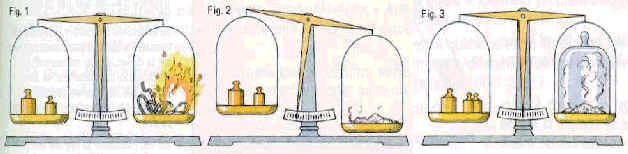
\includegraphics{lavoisier}
\end{figure}

\subsection{Ley de las Proporciones Definidas (Ley de Proust)}

Si en condiciones cuidadosamente controladas, hacemos reaccionar por ejemplo, 10 g de cloro con 10 g de sodio, podrá probarse que los 10 g de cloro no reaccionan con todo el sodio, sino solo con una porción de él (6,484 g exactamente) quedándose el exceso sin reaccionar. Según la experiencia, el cloro y el sodio han reaccionado en la proporción en peso:\\

\begin{center}
	$\frac{m_{Na}}{m_{Cl}}=\frac{6,484}{10}$
\end{center}

\begin{law}[Ley de Proust]
	Cuando dos o más elementos se combinan para formar un determinado compuesto lo hacen en una relación en peso constante independientemente del proceso seguido para formarlo.
\end{law}

Esta ley fue enunciada por \emph{Louis Proust} en 1799, y atacada por \emph{C. L. Berthollet}, quién creía que la composición de un compuesto variaba según el método por el que se había preparado.\\

Modernamente se conocen compuestos sólidos que no cumplen la ley de las proporciones definidas (óxidos y sulfuras de elementos de transición), y se les llama compuestos no estequiométricos o \emph{Compuestos Berthóllidos}.\\

Podemos decir por tanto que:

\begin{center}
		$\frac{m_{Na}}{m_{Cl}}=\frac{6,484}{10}=\frac{12,968}{20}=\frac{4,934}{7,61}=cte$
\end{center}

Cada muestra de sal común descompuesta nos arrojará invariablemente un 39,34 \% de sodio y un 60,66 \% de cloro (relación 6,484/10)

\subsection{Ley de las Proporciones Múltiples (Ley de Dalton)}

La ley anterior no excluye la posibilidad de que dos sustancias puedan formar compuestos diferentes si varían las condiciones experimentales. De hecho, esto es lo que sucede, por ejemplo, con el oxígeno y el hierro o el cobre o el carbono, que dependiendo de las condiciones de la experiencia se originan óxidos diferentes. Para cada proceso individual, se cumple, por supuesto la ley de Proust, sin embargo, cabe hablar de otra más general que incluye estos casos. Veamos un ejemplo:\\

Al hacer reaccionar un gramo de oxígeno con cobre, la cantidad de éste consumida es exactamente 3,971 g:

\begin{center}
	$Oxígeno (1 gr) + Cobre  (3,971 gr) \rightarrow Óxido de Cobre
	$ 
\end{center}

Pero en condiciones experimentales diferentes, un gramo de oxígeno puede reaccionar con 7,942 g de cobre para dar lugar a otro compuesto diferente:

\begin{center}
	$Oxígeno (1 gr) + Cobre (7,942 gr) \rightarrow Óxido de Cobre’ $
\end{center}

Si dividimos los gramos de cobre que en ambos casos se combinaron con la misma cantidad (un gramo) de oxígeno, veremos que resulta una relación muy sencilla:

\begin{center}
	$\frac{3,971}{7,942}=\frac{1}{2}$
\end{center}

Lo anterior es un ejemplo de la Ley de las Proporciones Múltiples enunciada en 1803 por \emph{J. Dalton}:\\

\begin{law}[Ley de Dalton de las Proporciones Múltiple]
	Las cantidades de un mismo elemento que se combinan con una cantidad fija de otro para formar varios compuestos están en la relación de los números enteros sencillos
\end{law}

\subsection{Ley de las Proporciones Equivalentes (Ley de Richter)}

Fue enunciada por primera vez por \emph{J.B. Richter} en 1792. Es de importancia para la historia de la química y el desarrollo del concepto de mol y de fórmula química más que para la química actual. Esta ley permite establecer el peso equivalente o peso-equivalente-gramo, que es la cantidad de un elemento o compuesto que reaccionará con una cantidad fija de una sustancia de referencia.\\

\begin{law}[Ley de Richter]
	
	Las masas de dos elementos diferentes que se combinan con una misma cantidad de un tercer elemento, guardan la misma relación que las masas de aquellos elementos cuando se combinan entre sí.
\end{law}

\section{Teoría Atómica de Dalton}

El Químico inglés \emph{John Dalton (1766-1844)} fue uno de los primeros que reflexionó sobre estas leyes empíricas y otras leyes sobre el comportamiento de los gases, llegando a la conclusión de que los elementos químicos deberían estar constituidos por partículas pequeñísimas e indivisibles a las que denominó átomos. Mucho tiempo antes que él, el griego \emph{Demócrito de Abdera} había propuesto esta misma denominación para explicar los constituyentes íntimos de la materia. Dalton adoptó el mismo término. La llamada \textbf{Teoría Atómica de Dalton} establecía como puntos fundamentales que:

\begin{itemize}
	\item Los elementos químicos están formados por partículas (átomos) que son indivisibles e inalterables en todo proceso químico.\\
	\item Todos los átomos de un mismo elemento son exactamente ¡guales entre sí y distintos a los átomos de otro elemento diferente.\\
	\item Los compuestos se originan por la unión intensa de átomos distintos en una proporción constante.
\end{itemize}

Con estas ideas, Dalton podía explicar las leyes ponderales conocidas. En efecto, si los átomos son inalterables y una reacción química no es más que la reordenación de átomos, deberá haber el mismo número de estos átomos en todo el proceso, por lo que la masa debería permanecer inalterada.

\section{Leyes Volumétricas}

Son un conjunto de leyes de naturaleza empírica que relaciona los volúmenes de gases que intervienen en una reacción química.

\subsection{Ley de los Volúmenes de Combinación de Gay-Lussac}

El químico francés \emph{Joseph Louis Gay-Lussac} (1778-1850) estudió las reacciones en las que intervenían gases, realizando sus estudios en reacciones a Presión y Temperatura constantes. Tras estudiar distintos tipos de reacciones químicas (siempre en fase gaseosa) llegó a la conclusión que ocurría algo análogo a la la Ley de Proust cuando se medían los distintos volúmenes de las sustancias intervinientes en la reacción.\\



\begin{law}[Ley de los Volúmenes de Combinación de Gay-Lussac]
	Los volúmenes de las sustancias gaseosas que intervienen en una reacción química, medidos en las mismas condiciones de presión y temperatura, están en relación de números enteros sencillos.
\end{law}

\begin{center}
	\textbf{Cuando Dalton recibió esta información encontró algo que no cuadraba con su teoría de átomos indivisibles.}\\
\end{center}

Si la reacción de formación de agua se da en esas proporciones es evidente que la fórmula del agua no es HO, sino H2O. Esto fue aceptado por Dalton (es una manera de determinar fórmulas) y supuso la corrección de la escala de masas atómicas relativas: el átomo de oxígeno tiene una masa igual a la de 16 átomos de hidrógeno.\\

Dalton aceptó que dos átomos de hidrógeno se combinaban con un átomo de oxígeno. Pero esta combinación debía producir una partícula (él la llamó átomo- compuesto) de agua, y por tanto, el volumen de agua obtenido debía ser un litro. Como Gay-Lussac informó de la obtención de dos litros de vapor de agua, Dalton supuso que tales medidas no podían ser correctas. Sin embargo, los datos obtenidos en el laboratorio eran claros: Gay-Lussac no estaba equivocado, un litro de oxígeno se combina con dos litros de hidrógeno y produce dos litros de vapor de agua. La solución vendría de otro químico genial: \textbf{Amadeo Avogadro}.

\subsection{Hipótesis de Avogadro}

En sus hipótesis Avogadro sugiere que las partículas de los gases son en realidad de dimensiones mucho menores que el volumen del recipiente que las contienen, de forma que estas no están en reposo como creía Dalton, sino están muy separadas en continuo movimiento. Sin esta condición no parecería lógico que moléculas grandes o pequeñas ocuparan el mismo volumen. Pronto se comprobó que las partículas de los gases elementales son moléculas diatómicas y la primera utilidad fue la determinación de fórmulas de compuestos y, por tanto, la determinación de las masas atómicas relativas correctas.\\

Según Avogadro:

\begin{itemize}
	\item Cada molécula de agua debe tener, como mínimo, un átomo de oxígeno. Si el volumen de agua que se obtiene es el doble que el de oxígeno, la molécula de oxígeno debe ser diatómica, para que cada molécula origine los átomos que permitan formar dos moléculas de agua.\\
	\item Como el volumen de agua es el mismo que el de hidrógeno, debe haber el mismo número de moléculas de cada uno.
\end{itemize}

\begin{law}[Hipótesis de Avogadro]
	En condiciones iguales de presión y temperatura, volúmenes iguales de gases diferentes tienen el mismo número de moléculas....
\end{law}

\section{Concepto de Mol}

Determinar la masa de un átomo o de una molécula es evidentemente imposible usando las balanzas, de ahí que los químicos hayan decidido definir una "nueva" unidad para medir la masa de átomos y moléculas. A esa unidad se la denomina unidad de masa atómica (uma) y ya que el hidrógeno se ha comprobado que es el elemento de menos masa es lógico definirlo como unidad, definirlo como uma.\\

Así en una primera aproximación diremos que la unidad de masa atómica es simplemente la masa de un átomo de hidrógeno. De modo que si decimos que, por ejemplo, el carbono tiene de masa atómica 12 urna, con ello estamos diciendo que un átomo de carbono pesa 12 veces más que un átomo de hidrógeno, o si decimos que la molécula de agua pesa 18 urna, decimos que una molécula de agua pesa 18 veces más que un átomo de hidrógeno, y así sucesivamente.\\

Lógicamente la masa de una molécula (masa molecular) se obtendrá por la suma de las masas atómicas de cada uno de los elementos que la forman. Esos datos de masas atómicas vienen recogidas en la tabla periódica. Con todo, en los laboratorios las balanzas no miden uma, sino gramos, de ahí que haga falta hallar una relación entre ambas escalas.\\


Mil moléculas (o átomos) de cualquier especie es aún un número muy pequeño para poder pesarse en la balanza, pero todo es cuestión de escoger un número muy grande de moléculas (o átomos) que podamos pesar. Lógicamente, 1000 átomos de carbono, por ejemplo, pesarían en uma $12\cdot 1000$. Si en lugar de elegir mil elegimos $10^{23}$ resulta que ese es un número ya muy muy grande. Si escogemos $6,02\cdot10^{23}$ átomos de carbono, éstos pesarán $12\cdot6,02\cdot10^23$ uma, pero curiosamente, al poner todos esos átomos sobre la balanza, "curiosamente" pesan 12 gramos.\\

\begin{definition}[Mol]
	El mol corresponde con la cantidad de materia que contiene $6.022\cdot10^{23}$ átomos o moléculas de una determinada sustancia
\end{definition}

Esa es la ventaja de elegir “ese número tan raro", que \textbf{la masa en gramos de la especie elegida coincide numéricamente con la masa en uma}.\\
A ese “número tan raro” se le conoce con el nombre de \textbf{Número de Avogadro}:\\

\begin{center}
$N_A=6,02\cdot10^{23}$
\end{center}
Por todo lo anteriormente expuesto aquí, existe una manera de calcular la equivalencia entre gramos y moles de una substancia:

\begin{definition}[Definición de Mol]
	Se define el Mol como los gramos de una determinada sustancia dividida por su masa molecular:
	\begin{align}
		& n=\frac{gr}{M_m}
	\end{align}
\end{definition}

\begin{exercise}
	Calcula los moles de moléculas de Ácido Sulfúrico contenidas en 100 gr de dicha substancia. Calcula también los moles y el número de átomos de oxígeno.
	
\end{exercise}